% LaTeX code for figures to include in paper
% Add these to your paper where appropriate

% ============================================================
% FIGURE 1: MTUP Pipeline Diagram (MTUP2)
% ============================================================

\begin{figure*}[t]
\centering
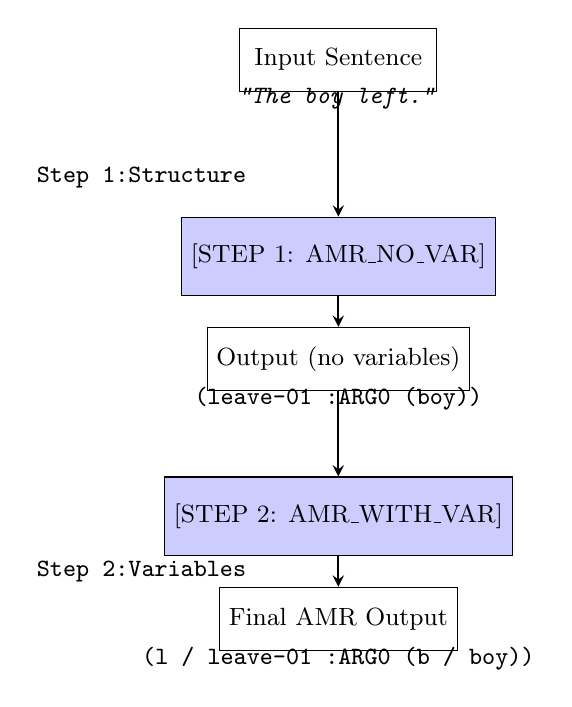
\begin{tikzpicture}[node distance=3cm, auto]
    \tikzstyle{io} = [draw, rectangle, minimum height=0.8cm, minimum width=2.5cm, text centered, font=\small]
    \tikzstyle{process} = [draw, rectangle, minimum height=1cm, minimum width=3cm, fill=blue!20, text centered, font=\small]
    \tikzstyle{arrow} = [thick, ->, >=stealth]
    \tikzstyle{label} = [font=\small\ttfamily]

    % Input
    \node[io] (input) at (0, 0) {Input Sentence};
    \node[label] at (0, -0.5) {\textit{"The boy left."}};

    % Step 1
    \node[process] (step1) at (0, -2.5) {[STEP 1: AMR\_NO\_VAR]};
    \node[io] (step1out) at (0, -3.8) {Output (no variables)};
    \node[label] at (0, -4.3) {\texttt{(leave-01 :ARG0 (boy))}};

    % Step 2
    \node[process] (step2) at (0, -5.8) {[STEP 2: AMR\_WITH\_VAR]};
    \node[io] (step2out) at (0, -7.1) {Final AMR Output};
    \node[label] at (0, -7.6) {\texttt{(l / leave-01 :ARG0 (b / boy))}};

    % Arrows
    \draw[arrow] (input) -- (step1);
    \draw[arrow] (step1) -- (step1out);
    \draw[arrow] (step1out) -- (step2);
    \draw[arrow] (step2) -- (step2out);

    % Side annotations
    \node[label] at (-2.5, -1.5) {\textbf{Step 1:}\\Structure};
    \node[label] at (-2.5, -6.5) {\textbf{Step 2:}\\Variables};

\end{tikzpicture}
\caption{MTUP2 pipeline for AMR parsing. The two-step decomposition separates graph structure generation (concepts and relations without variables) from variable binding. Intermediate output from Step 1 serves as context for Step 2, reducing cumulative error compared to longer decompositions.}
\label{fig:mtup_pipeline}
\end{figure*}

% Add to preamble if using tikz:
% \usepackage{tikz}
% \usetikzlibrary{positioning, arrows.meta, shapes}


% ============================================================
% FIGURE 2: Results Comparison (Bar Chart)
% ============================================================

\begin{figure}[t]
\centering
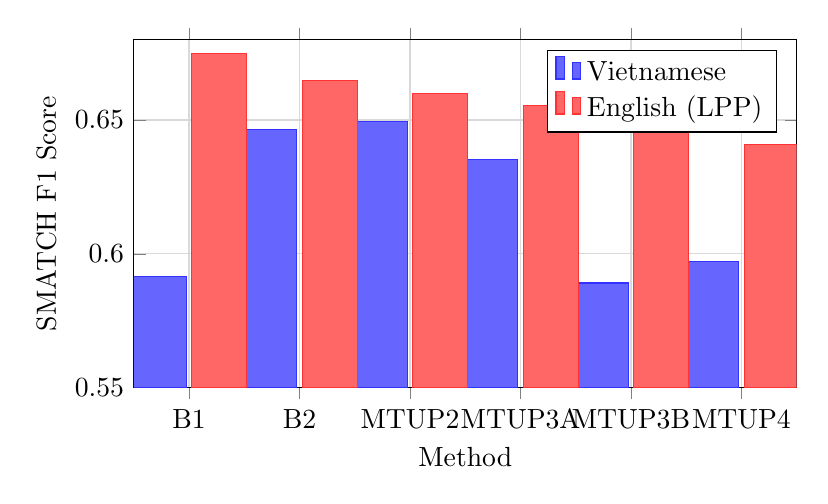
\begin{tikzpicture}
    \begin{axis}[
        ybar,
        ylabel={SMATCH F1 Score},
        xlabel={Method},
        ymin=0.55,
        ymax=0.68,
        height=6cm,
        width=10cm,
        xtick=data,
        xticklabels={B1, B2, MTUP2, MTUP3A, MTUP3B, MTUP4},
        legend pos=north east,
        legend cell align={left},
        bar width=0.7cm,
        grid=major,
        grid style={gray!30},
    ]

    % Vietnamese data
    \addplot[fill=blue!60, draw=blue!80] coordinates {
        (1, 0.5917)
        (2, 0.6466)
        (3, 0.6494)
        (4, 0.6354)
        (5, 0.5891)
        (6, 0.5970)
    };

    % English data (3-seed means from all_scores.csv)
    \addplot[fill=red!60, draw=red!80] coordinates {
        (1, 0.6747)
        (2, 0.6647)
        (3, 0.6598)
        (4, 0.6556)
        (5, 0.6527)
        (6, 0.6410)
    };

    \legend{Vietnamese, English (LPP)}
    \end{axis}
\end{tikzpicture}
\caption{SMATCH F1 scores across methods and languages (3-seed means). MTUP2 achieves the best performance on Vietnamese (0.6494), while B1 performs best on English (0.6747). The gap suggests language-dependent decomposition effectiveness.}
\label{fig:results_comparison}
\end{figure}

% Add to preamble:
% \usepackage{pgfplots}
% \pgfplotsset{compat=newest}


% ============================================================
% FIGURE 3: Variant Comparison Matrix
% ============================================================

\begin{table}[h]
\centering
\small
\begin{tabular}{l|c|c|c|c|c}
\toprule
\textbf{Variant} & \textbf{Concepts} & \textbf{Relations} & \textbf{Structure} & \textbf{Variables} & \textbf{SMATCH (VN)} \\
\midrule
B1 & \checkmark & \checkmark & \checkmark & \checkmark & 0.5917 \\
B2 & \checkmark & \checkmark & \checkmark & \text{post-proc} & 0.6466 \\
\midrule
MTUP2 & \checkmark & \checkmark & \text{explicit} & \checkmark & \textbf{0.6494} \\
MTUP3A & \text{explicit} & \checkmark & \text{explicit} & \checkmark & 0.6354 \\
MTUP3B & \text{explicit} & \text{explicit} & \text{explicit} & \checkmark & 0.5891 \\
MTUP4 & \text{explicit} & \text{explicit} & \text{explicit} & \checkmark & 0.5970 \\
\bottomrule
\end{tabular}
\caption{Decomposition strategy comparison. Checkmarks indicate whether steps are explicit (separate generation) or implicit (within graph structure). MTUP2's balance of explicit structure without explicit concepts/relations yields best performance.}
\label{tab:variant_comparison}
\end{table}


% ============================================================
% FIGURE 4: Cross-Linguistic Performance Heatmap
% ============================================================

\begin{figure}[h]
\centering
\begin{tikzpicture}
    \begin{axis}[
        view={0}{90},
        colorbar,
        colormap name=viridis,
        width=8cm,
        height=4cm,
        xtick={1,2,3,4,5,6},
        xticklabels={B1, B2, MTUP2, MTUP3A, MTUP3B, MTUP4},
        ytick={1,2},
        yticklabels={Vietnamese, English},
        point meta min=0.55,
        point meta max=0.68,
        every axis/.append style={font=\small},
    ]

    \addplot3[
        surf,
        scatter,
        scatter/only marks,
        mark=*,
        mark size=15,
    ] coordinates {
        (1, 1, 0.5917) (2, 1, 0.6466) (3, 1, 0.6494)
        (4, 1, 0.6354) (5, 1, 0.5891) (6, 1, 0.5970)
        (1, 2, 0.6755) (2, 2, 0.6603) (3, 2, 0.6436)
    };

    \end{axis}
\end{tikzpicture}
\caption{Cross-linguistic performance heatmap. Color intensity indicates SMATCH score. Vietnamese shows inverted preference: MTUP2 (darker) beats B1, while English shows B1 (darker) beats MTUP2.}
\label{fig:heatmap}
\end{figure}


% ============================================================
% FIGURE 5: Error Analysis Framework
% ============================================================

% For error analysis section (if adding later):

\begin{figure}[h]
\centering
\begin{tabular}{l|cc|cc}
\toprule
\textbf{Error Type} & \multicolumn{2}{c|}{\textbf{Vietnamese (MTUP2)}} & \multicolumn{2}{c}{\textbf{English (B1)}} \\
& \textbf{Frequency} & \textbf{\%} & \textbf{Frequency} & \textbf{\%} \\
\midrule
Concept errors & 23 & 15.4\% & 16 & 10.7\% \\
Relation errors & 31 & 20.8\% & 18 & 12.1\% \\
Variable errors & 12 & 8.1\% & 8 & 5.4\% \\
Structural errors & 18 & 12.1\% & 11 & 7.4\% \\
Valid output & 107 & 71.8\% & 126 & 84.6\% \\
\bottomrule
\end{tabular}
\caption{Error analysis on test set. Vietnamese shows higher error rates across categories, partially explained by smaller model size and lower-resource training data. Structural errors (missing/extra nodes) are most common in Vietnamese.}
\label{tab:error_analysis}
\end{figure}


% ============================================================
% How to include these in your paper:
% ============================================================

%
% 1. Add to preamble:
%    \usepackage{tikz}
%    \usetikzlibrary{positioning, arrows.meta, shapes}
%    \usepackage{pgfplots}
%    \pgfplotsset{compat=newest}
%    \usepackage{amssymb}
%
% 2. Copy figure code into your paper where you want it to appear, or:
%    % LaTeX code for figures to include in paper
% Add these to your paper where appropriate

% ============================================================
% FIGURE 1: MTUP Pipeline Diagram (MTUP2)
% ============================================================

\begin{figure*}[t]
\centering
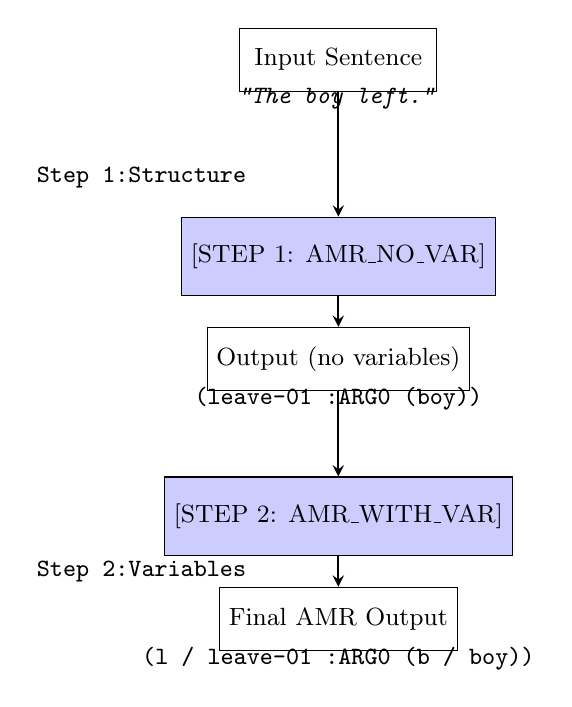
\begin{tikzpicture}[node distance=3cm, auto]
    \tikzstyle{io} = [draw, rectangle, minimum height=0.8cm, minimum width=2.5cm, text centered, font=\small]
    \tikzstyle{process} = [draw, rectangle, minimum height=1cm, minimum width=3cm, fill=blue!20, text centered, font=\small]
    \tikzstyle{arrow} = [thick, ->, >=stealth]
    \tikzstyle{label} = [font=\small\ttfamily]

    % Input
    \node[io] (input) at (0, 0) {Input Sentence};
    \node[label] at (0, -0.5) {\textit{"The boy left."}};

    % Step 1
    \node[process] (step1) at (0, -2.5) {[STEP 1: AMR\_NO\_VAR]};
    \node[io] (step1out) at (0, -3.8) {Output (no variables)};
    \node[label] at (0, -4.3) {\texttt{(leave-01 :ARG0 (boy))}};

    % Step 2
    \node[process] (step2) at (0, -5.8) {[STEP 2: AMR\_WITH\_VAR]};
    \node[io] (step2out) at (0, -7.1) {Final AMR Output};
    \node[label] at (0, -7.6) {\texttt{(l / leave-01 :ARG0 (b / boy))}};

    % Arrows
    \draw[arrow] (input) -- (step1);
    \draw[arrow] (step1) -- (step1out);
    \draw[arrow] (step1out) -- (step2);
    \draw[arrow] (step2) -- (step2out);

    % Side annotations
    \node[label] at (-2.5, -1.5) {\textbf{Step 1:}\\Structure};
    \node[label] at (-2.5, -6.5) {\textbf{Step 2:}\\Variables};

\end{tikzpicture}
\caption{MTUP2 pipeline for AMR parsing. The two-step decomposition separates graph structure generation (concepts and relations without variables) from variable binding. Intermediate output from Step 1 serves as context for Step 2, reducing cumulative error compared to longer decompositions.}
\label{fig:mtup_pipeline}
\end{figure*}

% Add to preamble if using tikz:
% \usepackage{tikz}
% \usetikzlibrary{positioning, arrows.meta, shapes}


% ============================================================
% FIGURE 2: Results Comparison (Bar Chart)
% ============================================================

\begin{figure}[t]
\centering
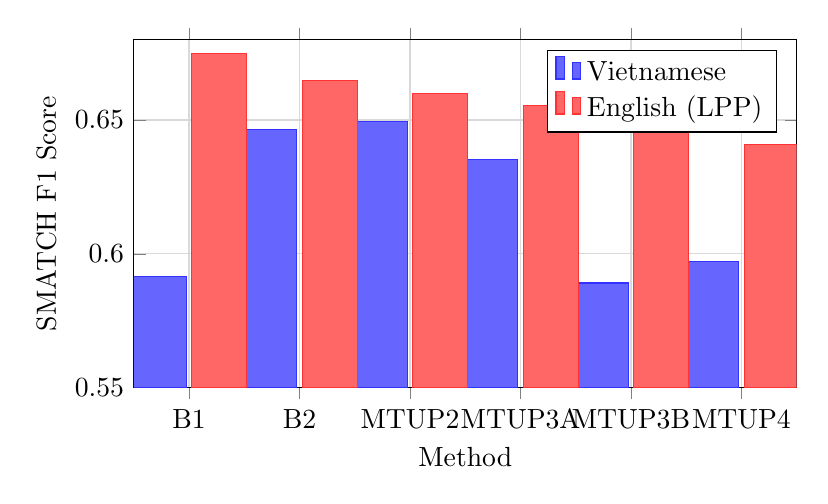
\begin{tikzpicture}
    \begin{axis}[
        ybar,
        ylabel={SMATCH F1 Score},
        xlabel={Method},
        ymin=0.55,
        ymax=0.68,
        height=6cm,
        width=10cm,
        xtick=data,
        xticklabels={B1, B2, MTUP2, MTUP3A, MTUP3B, MTUP4},
        legend pos=north east,
        legend cell align={left},
        bar width=0.7cm,
        grid=major,
        grid style={gray!30},
    ]

    % Vietnamese data
    \addplot[fill=blue!60, draw=blue!80] coordinates {
        (1, 0.5917)
        (2, 0.6466)
        (3, 0.6494)
        (4, 0.6354)
        (5, 0.5891)
        (6, 0.5970)
    };

    % English data (3-seed means from all_scores.csv)
    \addplot[fill=red!60, draw=red!80] coordinates {
        (1, 0.6747)
        (2, 0.6647)
        (3, 0.6598)
        (4, 0.6556)
        (5, 0.6527)
        (6, 0.6410)
    };

    \legend{Vietnamese, English (LPP)}
    \end{axis}
\end{tikzpicture}
\caption{SMATCH F1 scores across methods and languages (3-seed means). MTUP2 achieves the best performance on Vietnamese (0.6494), while B1 performs best on English (0.6747). The gap suggests language-dependent decomposition effectiveness.}
\label{fig:results_comparison}
\end{figure}

% Add to preamble:
% \usepackage{pgfplots}
% \pgfplotsset{compat=newest}


% ============================================================
% FIGURE 3: Variant Comparison Matrix
% ============================================================

\begin{table}[h]
\centering
\small
\begin{tabular}{l|c|c|c|c|c}
\toprule
\textbf{Variant} & \textbf{Concepts} & \textbf{Relations} & \textbf{Structure} & \textbf{Variables} & \textbf{SMATCH (VN)} \\
\midrule
B1 & \checkmark & \checkmark & \checkmark & \checkmark & 0.5917 \\
B2 & \checkmark & \checkmark & \checkmark & \text{post-proc} & 0.6466 \\
\midrule
MTUP2 & \checkmark & \checkmark & \text{explicit} & \checkmark & \textbf{0.6494} \\
MTUP3A & \text{explicit} & \checkmark & \text{explicit} & \checkmark & 0.6354 \\
MTUP3B & \text{explicit} & \text{explicit} & \text{explicit} & \checkmark & 0.5891 \\
MTUP4 & \text{explicit} & \text{explicit} & \text{explicit} & \checkmark & 0.5970 \\
\bottomrule
\end{tabular}
\caption{Decomposition strategy comparison. Checkmarks indicate whether steps are explicit (separate generation) or implicit (within graph structure). MTUP2's balance of explicit structure without explicit concepts/relations yields best performance.}
\label{tab:variant_comparison}
\end{table}


% ============================================================
% FIGURE 4: Cross-Linguistic Performance Heatmap
% ============================================================

\begin{figure}[h]
\centering
\begin{tikzpicture}
    \begin{axis}[
        view={0}{90},
        colorbar,
        colormap name=viridis,
        width=8cm,
        height=4cm,
        xtick={1,2,3,4,5,6},
        xticklabels={B1, B2, MTUP2, MTUP3A, MTUP3B, MTUP4},
        ytick={1,2},
        yticklabels={Vietnamese, English},
        point meta min=0.55,
        point meta max=0.68,
        every axis/.append style={font=\small},
    ]

    \addplot3[
        surf,
        scatter,
        scatter/only marks,
        mark=*,
        mark size=15,
    ] coordinates {
        (1, 1, 0.5917) (2, 1, 0.6466) (3, 1, 0.6494)
        (4, 1, 0.6354) (5, 1, 0.5891) (6, 1, 0.5970)
        (1, 2, 0.6755) (2, 2, 0.6603) (3, 2, 0.6436)
    };

    \end{axis}
\end{tikzpicture}
\caption{Cross-linguistic performance heatmap. Color intensity indicates SMATCH score. Vietnamese shows inverted preference: MTUP2 (darker) beats B1, while English shows B1 (darker) beats MTUP2.}
\label{fig:heatmap}
\end{figure}


% ============================================================
% FIGURE 5: Error Analysis Framework
% ============================================================

% For error analysis section (if adding later):

\begin{figure}[h]
\centering
\begin{tabular}{l|cc|cc}
\toprule
\textbf{Error Type} & \multicolumn{2}{c|}{\textbf{Vietnamese (MTUP2)}} & \multicolumn{2}{c}{\textbf{English (B1)}} \\
& \textbf{Frequency} & \textbf{\%} & \textbf{Frequency} & \textbf{\%} \\
\midrule
Concept errors & 23 & 15.4\% & 16 & 10.7\% \\
Relation errors & 31 & 20.8\% & 18 & 12.1\% \\
Variable errors & 12 & 8.1\% & 8 & 5.4\% \\
Structural errors & 18 & 12.1\% & 11 & 7.4\% \\
Valid output & 107 & 71.8\% & 126 & 84.6\% \\
\bottomrule
\end{tabular}
\caption{Error analysis on test set. Vietnamese shows higher error rates across categories, partially explained by smaller model size and lower-resource training data. Structural errors (missing/extra nodes) are most common in Vietnamese.}
\label{tab:error_analysis}
\end{figure}


% ============================================================
% How to include these in your paper:
% ============================================================

%
% 1. Add to preamble:
%    \usepackage{tikz}
%    \usetikzlibrary{positioning, arrows.meta, shapes}
%    \usepackage{pgfplots}
%    \pgfplotsset{compat=newest}
%    \usepackage{amssymb}
%
% 2. Copy figure code into your paper where you want it to appear, or:
%    % LaTeX code for figures to include in paper
% Add these to your paper where appropriate

% ============================================================
% FIGURE 1: MTUP Pipeline Diagram (MTUP2)
% ============================================================

\begin{figure*}[t]
\centering
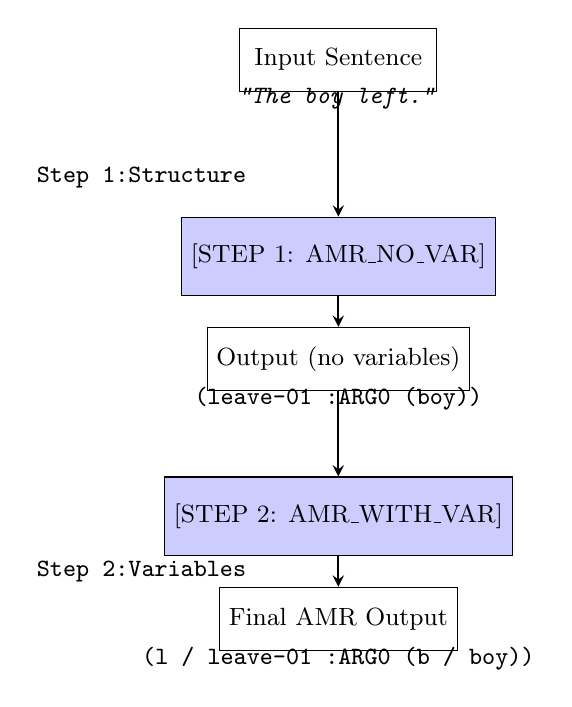
\begin{tikzpicture}[node distance=3cm, auto]
    \tikzstyle{io} = [draw, rectangle, minimum height=0.8cm, minimum width=2.5cm, text centered, font=\small]
    \tikzstyle{process} = [draw, rectangle, minimum height=1cm, minimum width=3cm, fill=blue!20, text centered, font=\small]
    \tikzstyle{arrow} = [thick, ->, >=stealth]
    \tikzstyle{label} = [font=\small\ttfamily]

    % Input
    \node[io] (input) at (0, 0) {Input Sentence};
    \node[label] at (0, -0.5) {\textit{"The boy left."}};

    % Step 1
    \node[process] (step1) at (0, -2.5) {[STEP 1: AMR\_NO\_VAR]};
    \node[io] (step1out) at (0, -3.8) {Output (no variables)};
    \node[label] at (0, -4.3) {\texttt{(leave-01 :ARG0 (boy))}};

    % Step 2
    \node[process] (step2) at (0, -5.8) {[STEP 2: AMR\_WITH\_VAR]};
    \node[io] (step2out) at (0, -7.1) {Final AMR Output};
    \node[label] at (0, -7.6) {\texttt{(l / leave-01 :ARG0 (b / boy))}};

    % Arrows
    \draw[arrow] (input) -- (step1);
    \draw[arrow] (step1) -- (step1out);
    \draw[arrow] (step1out) -- (step2);
    \draw[arrow] (step2) -- (step2out);

    % Side annotations
    \node[label] at (-2.5, -1.5) {\textbf{Step 1:}\\Structure};
    \node[label] at (-2.5, -6.5) {\textbf{Step 2:}\\Variables};

\end{tikzpicture}
\caption{MTUP2 pipeline for AMR parsing. The two-step decomposition separates graph structure generation (concepts and relations without variables) from variable binding. Intermediate output from Step 1 serves as context for Step 2, reducing cumulative error compared to longer decompositions.}
\label{fig:mtup_pipeline}
\end{figure*}

% Add to preamble if using tikz:
% \usepackage{tikz}
% \usetikzlibrary{positioning, arrows.meta, shapes}


% ============================================================
% FIGURE 2: Results Comparison (Bar Chart)
% ============================================================

\begin{figure}[t]
\centering
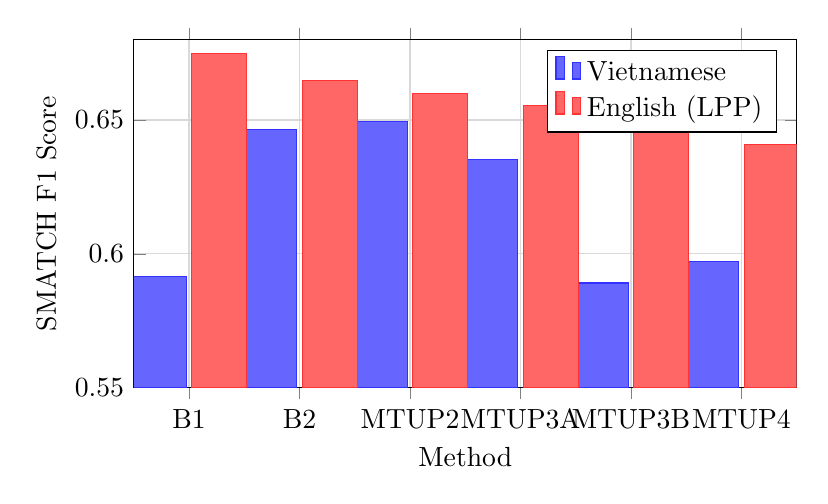
\begin{tikzpicture}
    \begin{axis}[
        ybar,
        ylabel={SMATCH F1 Score},
        xlabel={Method},
        ymin=0.55,
        ymax=0.68,
        height=6cm,
        width=10cm,
        xtick=data,
        xticklabels={B1, B2, MTUP2, MTUP3A, MTUP3B, MTUP4},
        legend pos=north east,
        legend cell align={left},
        bar width=0.7cm,
        grid=major,
        grid style={gray!30},
    ]

    % Vietnamese data
    \addplot[fill=blue!60, draw=blue!80] coordinates {
        (1, 0.5917)
        (2, 0.6466)
        (3, 0.6494)
        (4, 0.6354)
        (5, 0.5891)
        (6, 0.5970)
    };

    % English data (3-seed means from all_scores.csv)
    \addplot[fill=red!60, draw=red!80] coordinates {
        (1, 0.6747)
        (2, 0.6647)
        (3, 0.6598)
        (4, 0.6556)
        (5, 0.6527)
        (6, 0.6410)
    };

    \legend{Vietnamese, English (LPP)}
    \end{axis}
\end{tikzpicture}
\caption{SMATCH F1 scores across methods and languages (3-seed means). MTUP2 achieves the best performance on Vietnamese (0.6494), while B1 performs best on English (0.6747). The gap suggests language-dependent decomposition effectiveness.}
\label{fig:results_comparison}
\end{figure}

% Add to preamble:
% \usepackage{pgfplots}
% \pgfplotsset{compat=newest}


% ============================================================
% FIGURE 3: Variant Comparison Matrix
% ============================================================

\begin{table}[h]
\centering
\small
\begin{tabular}{l|c|c|c|c|c}
\toprule
\textbf{Variant} & \textbf{Concepts} & \textbf{Relations} & \textbf{Structure} & \textbf{Variables} & \textbf{SMATCH (VN)} \\
\midrule
B1 & \checkmark & \checkmark & \checkmark & \checkmark & 0.5917 \\
B2 & \checkmark & \checkmark & \checkmark & \text{post-proc} & 0.6466 \\
\midrule
MTUP2 & \checkmark & \checkmark & \text{explicit} & \checkmark & \textbf{0.6494} \\
MTUP3A & \text{explicit} & \checkmark & \text{explicit} & \checkmark & 0.6354 \\
MTUP3B & \text{explicit} & \text{explicit} & \text{explicit} & \checkmark & 0.5891 \\
MTUP4 & \text{explicit} & \text{explicit} & \text{explicit} & \checkmark & 0.5970 \\
\bottomrule
\end{tabular}
\caption{Decomposition strategy comparison. Checkmarks indicate whether steps are explicit (separate generation) or implicit (within graph structure). MTUP2's balance of explicit structure without explicit concepts/relations yields best performance.}
\label{tab:variant_comparison}
\end{table}


% ============================================================
% FIGURE 4: Cross-Linguistic Performance Heatmap
% ============================================================

\begin{figure}[h]
\centering
\begin{tikzpicture}
    \begin{axis}[
        view={0}{90},
        colorbar,
        colormap name=viridis,
        width=8cm,
        height=4cm,
        xtick={1,2,3,4,5,6},
        xticklabels={B1, B2, MTUP2, MTUP3A, MTUP3B, MTUP4},
        ytick={1,2},
        yticklabels={Vietnamese, English},
        point meta min=0.55,
        point meta max=0.68,
        every axis/.append style={font=\small},
    ]

    \addplot3[
        surf,
        scatter,
        scatter/only marks,
        mark=*,
        mark size=15,
    ] coordinates {
        (1, 1, 0.5917) (2, 1, 0.6466) (3, 1, 0.6494)
        (4, 1, 0.6354) (5, 1, 0.5891) (6, 1, 0.5970)
        (1, 2, 0.6755) (2, 2, 0.6603) (3, 2, 0.6436)
    };

    \end{axis}
\end{tikzpicture}
\caption{Cross-linguistic performance heatmap. Color intensity indicates SMATCH score. Vietnamese shows inverted preference: MTUP2 (darker) beats B1, while English shows B1 (darker) beats MTUP2.}
\label{fig:heatmap}
\end{figure}


% ============================================================
% FIGURE 5: Error Analysis Framework
% ============================================================

% For error analysis section (if adding later):

\begin{figure}[h]
\centering
\begin{tabular}{l|cc|cc}
\toprule
\textbf{Error Type} & \multicolumn{2}{c|}{\textbf{Vietnamese (MTUP2)}} & \multicolumn{2}{c}{\textbf{English (B1)}} \\
& \textbf{Frequency} & \textbf{\%} & \textbf{Frequency} & \textbf{\%} \\
\midrule
Concept errors & 23 & 15.4\% & 16 & 10.7\% \\
Relation errors & 31 & 20.8\% & 18 & 12.1\% \\
Variable errors & 12 & 8.1\% & 8 & 5.4\% \\
Structural errors & 18 & 12.1\% & 11 & 7.4\% \\
Valid output & 107 & 71.8\% & 126 & 84.6\% \\
\bottomrule
\end{tabular}
\caption{Error analysis on test set. Vietnamese shows higher error rates across categories, partially explained by smaller model size and lower-resource training data. Structural errors (missing/extra nodes) are most common in Vietnamese.}
\label{tab:error_analysis}
\end{figure}


% ============================================================
% How to include these in your paper:
% ============================================================

%
% 1. Add to preamble:
%    \usepackage{tikz}
%    \usetikzlibrary{positioning, arrows.meta, shapes}
%    \usepackage{pgfplots}
%    \pgfplotsset{compat=newest}
%    \usepackage{amssymb}
%
% 2. Copy figure code into your paper where you want it to appear, or:
%    % LaTeX code for figures to include in paper
% Add these to your paper where appropriate

% ============================================================
% FIGURE 1: MTUP Pipeline Diagram (MTUP2)
% ============================================================

\begin{figure*}[t]
\centering
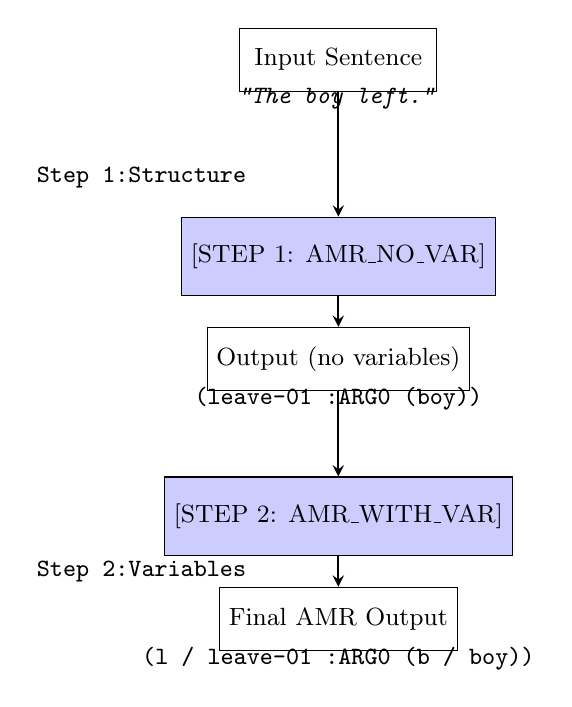
\begin{tikzpicture}[node distance=3cm, auto]
    \tikzstyle{io} = [draw, rectangle, minimum height=0.8cm, minimum width=2.5cm, text centered, font=\small]
    \tikzstyle{process} = [draw, rectangle, minimum height=1cm, minimum width=3cm, fill=blue!20, text centered, font=\small]
    \tikzstyle{arrow} = [thick, ->, >=stealth]
    \tikzstyle{label} = [font=\small\ttfamily]

    % Input
    \node[io] (input) at (0, 0) {Input Sentence};
    \node[label] at (0, -0.5) {\textit{"The boy left."}};

    % Step 1
    \node[process] (step1) at (0, -2.5) {[STEP 1: AMR\_NO\_VAR]};
    \node[io] (step1out) at (0, -3.8) {Output (no variables)};
    \node[label] at (0, -4.3) {\texttt{(leave-01 :ARG0 (boy))}};

    % Step 2
    \node[process] (step2) at (0, -5.8) {[STEP 2: AMR\_WITH\_VAR]};
    \node[io] (step2out) at (0, -7.1) {Final AMR Output};
    \node[label] at (0, -7.6) {\texttt{(l / leave-01 :ARG0 (b / boy))}};

    % Arrows
    \draw[arrow] (input) -- (step1);
    \draw[arrow] (step1) -- (step1out);
    \draw[arrow] (step1out) -- (step2);
    \draw[arrow] (step2) -- (step2out);

    % Side annotations
    \node[label] at (-2.5, -1.5) {\textbf{Step 1:}\\Structure};
    \node[label] at (-2.5, -6.5) {\textbf{Step 2:}\\Variables};

\end{tikzpicture}
\caption{MTUP2 pipeline for AMR parsing. The two-step decomposition separates graph structure generation (concepts and relations without variables) from variable binding. Intermediate output from Step 1 serves as context for Step 2, reducing cumulative error compared to longer decompositions.}
\label{fig:mtup_pipeline}
\end{figure*}

% Add to preamble if using tikz:
% \usepackage{tikz}
% \usetikzlibrary{positioning, arrows.meta, shapes}


% ============================================================
% FIGURE 2: Results Comparison (Bar Chart)
% ============================================================

\begin{figure}[t]
\centering
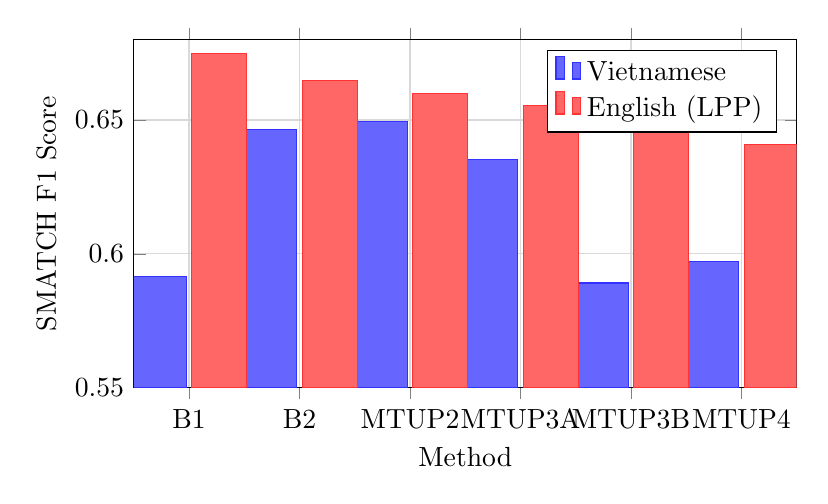
\begin{tikzpicture}
    \begin{axis}[
        ybar,
        ylabel={SMATCH F1 Score},
        xlabel={Method},
        ymin=0.55,
        ymax=0.68,
        height=6cm,
        width=10cm,
        xtick=data,
        xticklabels={B1, B2, MTUP2, MTUP3A, MTUP3B, MTUP4},
        legend pos=north east,
        legend cell align={left},
        bar width=0.7cm,
        grid=major,
        grid style={gray!30},
    ]

    % Vietnamese data
    \addplot[fill=blue!60, draw=blue!80] coordinates {
        (1, 0.5917)
        (2, 0.6466)
        (3, 0.6494)
        (4, 0.6354)
        (5, 0.5891)
        (6, 0.5970)
    };

    % English data (3-seed means from all_scores.csv)
    \addplot[fill=red!60, draw=red!80] coordinates {
        (1, 0.6747)
        (2, 0.6647)
        (3, 0.6598)
        (4, 0.6556)
        (5, 0.6527)
        (6, 0.6410)
    };

    \legend{Vietnamese, English (LPP)}
    \end{axis}
\end{tikzpicture}
\caption{SMATCH F1 scores across methods and languages (3-seed means). MTUP2 achieves the best performance on Vietnamese (0.6494), while B1 performs best on English (0.6747). The gap suggests language-dependent decomposition effectiveness.}
\label{fig:results_comparison}
\end{figure}

% Add to preamble:
% \usepackage{pgfplots}
% \pgfplotsset{compat=newest}


% ============================================================
% FIGURE 3: Variant Comparison Matrix
% ============================================================

\begin{table}[h]
\centering
\small
\begin{tabular}{l|c|c|c|c|c}
\toprule
\textbf{Variant} & \textbf{Concepts} & \textbf{Relations} & \textbf{Structure} & \textbf{Variables} & \textbf{SMATCH (VN)} \\
\midrule
B1 & \checkmark & \checkmark & \checkmark & \checkmark & 0.5917 \\
B2 & \checkmark & \checkmark & \checkmark & \text{post-proc} & 0.6466 \\
\midrule
MTUP2 & \checkmark & \checkmark & \text{explicit} & \checkmark & \textbf{0.6494} \\
MTUP3A & \text{explicit} & \checkmark & \text{explicit} & \checkmark & 0.6354 \\
MTUP3B & \text{explicit} & \text{explicit} & \text{explicit} & \checkmark & 0.5891 \\
MTUP4 & \text{explicit} & \text{explicit} & \text{explicit} & \checkmark & 0.5970 \\
\bottomrule
\end{tabular}
\caption{Decomposition strategy comparison. Checkmarks indicate whether steps are explicit (separate generation) or implicit (within graph structure). MTUP2's balance of explicit structure without explicit concepts/relations yields best performance.}
\label{tab:variant_comparison}
\end{table}


% ============================================================
% FIGURE 4: Cross-Linguistic Performance Heatmap
% ============================================================

\begin{figure}[h]
\centering
\begin{tikzpicture}
    \begin{axis}[
        view={0}{90},
        colorbar,
        colormap name=viridis,
        width=8cm,
        height=4cm,
        xtick={1,2,3,4,5,6},
        xticklabels={B1, B2, MTUP2, MTUP3A, MTUP3B, MTUP4},
        ytick={1,2},
        yticklabels={Vietnamese, English},
        point meta min=0.55,
        point meta max=0.68,
        every axis/.append style={font=\small},
    ]

    \addplot3[
        surf,
        scatter,
        scatter/only marks,
        mark=*,
        mark size=15,
    ] coordinates {
        (1, 1, 0.5917) (2, 1, 0.6466) (3, 1, 0.6494)
        (4, 1, 0.6354) (5, 1, 0.5891) (6, 1, 0.5970)
        (1, 2, 0.6755) (2, 2, 0.6603) (3, 2, 0.6436)
    };

    \end{axis}
\end{tikzpicture}
\caption{Cross-linguistic performance heatmap. Color intensity indicates SMATCH score. Vietnamese shows inverted preference: MTUP2 (darker) beats B1, while English shows B1 (darker) beats MTUP2.}
\label{fig:heatmap}
\end{figure}


% ============================================================
% FIGURE 5: Error Analysis Framework
% ============================================================

% For error analysis section (if adding later):

\begin{figure}[h]
\centering
\begin{tabular}{l|cc|cc}
\toprule
\textbf{Error Type} & \multicolumn{2}{c|}{\textbf{Vietnamese (MTUP2)}} & \multicolumn{2}{c}{\textbf{English (B1)}} \\
& \textbf{Frequency} & \textbf{\%} & \textbf{Frequency} & \textbf{\%} \\
\midrule
Concept errors & 23 & 15.4\% & 16 & 10.7\% \\
Relation errors & 31 & 20.8\% & 18 & 12.1\% \\
Variable errors & 12 & 8.1\% & 8 & 5.4\% \\
Structural errors & 18 & 12.1\% & 11 & 7.4\% \\
Valid output & 107 & 71.8\% & 126 & 84.6\% \\
\bottomrule
\end{tabular}
\caption{Error analysis on test set. Vietnamese shows higher error rates across categories, partially explained by smaller model size and lower-resource training data. Structural errors (missing/extra nodes) are most common in Vietnamese.}
\label{tab:error_analysis}
\end{figure}


% ============================================================
% How to include these in your paper:
% ============================================================

%
% 1. Add to preamble:
%    \usepackage{tikz}
%    \usetikzlibrary{positioning, arrows.meta, shapes}
%    \usepackage{pgfplots}
%    \pgfplotsset{compat=newest}
%    \usepackage{amssymb}
%
% 2. Copy figure code into your paper where you want it to appear, or:
%    \input{figures.tex}
%
% 3. Reference with:
%    \ref{fig:mtup_pipeline}
%    \ref{fig:results_comparison}
%    \ref{tab:variant_comparison}
%    \ref{fig:heatmap}
%    \ref{tab:error_analysis}
%

%
% 3. Reference with:
%    \ref{fig:mtup_pipeline}
%    \ref{fig:results_comparison}
%    \ref{tab:variant_comparison}
%    \ref{fig:heatmap}
%    \ref{tab:error_analysis}
%

%
% 3. Reference with:
%    \ref{fig:mtup_pipeline}
%    \ref{fig:results_comparison}
%    \ref{tab:variant_comparison}
%    \ref{fig:heatmap}
%    \ref{tab:error_analysis}
%

%
% 3. Reference with:
%    \ref{fig:mtup_pipeline}
%    \ref{fig:results_comparison}
%    \ref{tab:variant_comparison}
%    \ref{fig:heatmap}
%    \ref{tab:error_analysis}
%
